\documentclass{article}
\usepackage{tikz}
\begin{document}
\title{Hit Detection}
\author{31core}
\maketitle
\newpage
%----- Catalog -----
\tableofcontents
\newpage
\setlength{\parindent}{0em}
\section{Vector expression of Ray}
Any ray can be expressed using a point and a unit vector like this:
\begin{equation}
R = A + t\vec{B}
\end{equation}

\section{Hit detection of Sphere}
\subsection{Mathematical proof}
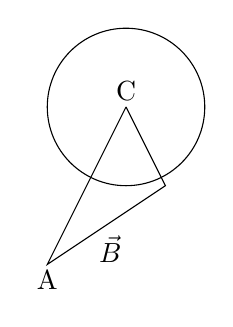
\begin{tikzpicture}
\draw (0, 0) circle (1);
\draw (0, 0)--(-1, -2)--(0.5, -1)--(0, 0);
\node at(-1, -2.2) {A};
\node at(-0.2, -1.8) {$\vec{B}$};
\node at(0, .2) {C};
\end{tikzpicture}

Because $\vec{CA} + t_d\vec{B}$ is perpendicular to $\vec{B}$, so we can get this equation.

$(\vec{CA} + t_d\vec{B})\vec{B} = 0$

We can get $t_d$ like this:

$t_d = \frac{ - \vec{CA} \cdot \vec{B} }{ \vec{B}^2 } = -\vec{CA} \cdot  \vec{B}$

Then calculate the distance from the center of the sphere to the ray:

$d = |\vec{CA} + t_d\vec{B}|$

Finally, calculate the $t$.

$t = \frac{|t_d\vec{B}| - \sqrt{R^2 - d^2}}{|\vec{B}|} = t_d - \sqrt{R^2 - d^2}$

If $d \leq R$ and $t \textgreater 0$, the ray do hit the sphere.

\subsection{Final formula}
\begin{equation}
t_d = -\vec{CA} \cdot  \vec{B}
\end{equation}
\begin{equation}
d = |\vec{CA} + t_d\vec{B}|
\end{equation}
\begin{equation}
t = t_d - \sqrt{R^2 - d^2}
\end{equation}

\section{Hit detection of Plane}

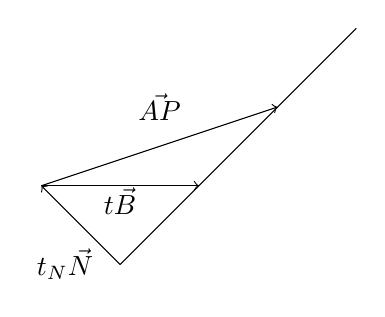
\begin{tikzpicture}
\draw (0, 0)--(3, 3);
% ray
\node at(0, 0.8) {$t\vec{B}$};
\draw[->] (-1, 1)--(1, 1);
% normal vector
\node at(-0.7, 0) {$t_N\vec{N}$};
\draw[->] (0, 0)--(-1, 1);
%AP vector
\node at(0.5, 2) {$\vec{AP}$};
\draw[->] (-1, 1)--(2, 2);
\end{tikzpicture}

$
(\vec{AP} + t_N\vec{N})\vec{N} = 0
\rightarrow
t_N = \frac{-\vec(AP)\vec{N}}{\vec{N}^2} = -\vec(AP)\vec{N}
$

$
(t_N\vec{N} + t\vec{B})\vec{N} = 0
\rightarrow
t = \frac{-t_N\vec{N}^2}{\vec{B}\vec{N}} = -\frac{t_N}{\vec{B}\vec{N}}
$

\subsection{Final formula}
\begin{equation}
t_N = -\vec{AP}\vec{N}
\end{equation}
\begin{equation}
t = -\frac{t_N}{\vec{B}\vec{N}}
\end{equation}

\section{Hit detection of Triangle}
\subsection{Mathematical proof}
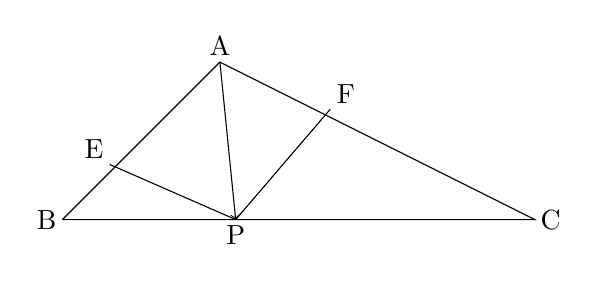
\begin{tikzpicture}
\draw (-2, 0)--(0, 2)--(4, 0)--(-2, 0);
\node at (0.2, -0.2) {P};
\draw[->] (0, 2)--(0.2, 0);
\node at (0, 2 + 0.2) {A};
\node at (-2 - 0.2, 0) {B};
\node at (4 + 0.2, 0) {C};

\node at (-1.4 - 0.2, 0.7 + 0.2) {E};
\draw (0.2, 0)--(-1.4, 0.7);
\node at (1.4 + 0.2, 1.4 + 0.2) {F};
\draw (0.2, 0)--(1.4, 1.4);
\end{tikzpicture}

$\vec{AP} = t_1\vec{AB} + t_2\vec{AC}$

$\vec{FP} = t_1\vec{AB}$

$
\vec{AF} = t_2\vec{AC}
\rightarrow
\vec{FC} = (1 - t_2)\vec{AC}
$

$
\frac{|\vec{FC}|}{|\vec{FP}|} = \frac{|(1 - t_2)\vec{AC}|}{|t_1\vec{AB}|} = \frac{|\vec{AC}|}{|\vec{AB}|}
$

$t_1 + t_2 = 1$

\section{Reflection of Ray}
\subsection{Mathematical proof}
$-\vec{A} + \vec{B} = t\vec{N}$

$(\frac{t}{2}\vec{B} + \vec{A})\vec{N} = 0$

$t = -\frac{2\vec{A}^2}{\vec{N} \cdot \vec{A}} = -\frac{2}{\vec{N} \cdot \vec{A}}$

\subsection{Final formula}
\begin{equation}
t = -\frac{2}{\vec{N} \cdot \vec{A}}
\end{equation}
\begin{equation}
\vec{B} = t\vec{N} + \vec{A}
\end{equation}

\section{Refraction of Ray}
\subsection{Mathematical proof}
\begin{tikzpicture}
%vector A
\node at(-1, 1) {$\vec{A}$};
\draw[->] (-1, 2)--(0, 0);
%normal vector
\draw[->] (0, 0)--(0, 2);
\draw[->] (0, -2)--(0, 0);
\draw (-2, 0)--(2, 0);
%vector B
\node at(0.6, -1) {$\vec{B}$};
\draw[->] (0, 0)--(0.6, -2);
%vector C
\node at(-0.5, 2.2) {$\vec{C}$};
\draw[->] (-1, 2)--(0, 2);
%vector D
\node at(0.3, -2.2) {$\vec{D}$};
\draw[->] (0, -2)--(0.6, -2);
\end{tikzpicture}

$
(\vec{A} + t\vec{N})\vec{N} = 0
\rightarrow
t = -\frac{\vec{A} \cdot \vec{N}}{\vec{N}^2}
=
-\vec{A} \cdot \vec{N}
$

Express $\vec{C}$ $\vec{D}$ that are perpendicular to $\vec{N}$:

$\vec{C} = \vec{A} + t\vec{N}$

$\vec{D} = \vec{B} + t\vec{N}$

Then we express refraction rate(n) with $\vec{A}$, $\vec{B}$, $\vec{C}$ and $\vec{D}$:

$
\frac{sin<-\vec{A}, \vec{N}>}{sin<\vec{B}, \vec{N}>}
=
\frac{\frac{|\vec{C}|}{|\vec{A}|}}{\frac{|\vec{D}|}{|\vec{B}|}} = n
\rightarrow
\vec{D} = \frac{|\vec{D}|}{|\vec{C}|} \cdot \vec{C}
=
\frac{\vec{C}}{n}
$

\subsection{Final formula}
\begin{equation}
t = -\vec{A} \cdot \vec{N}
\end{equation}

\begin{equation}
\vec{C} = \vec{A} + t\vec{N}
\end{equation}

\begin{equation}
\vec{B} = \frac{\vec{C}}{n} - t\vec{N}
\end{equation}
\end{document}
